\documentclass{article}

\usepackage{PRIMEarxiv}

\usepackage[utf8]{inputenc} % allow utf-8 input
\usepackage[T1]{fontenc}    % use 8-bit T1 fonts
\usepackage{hyperref}       % hyperlinks
\usepackage{url}            % simple URL typesetting
\usepackage{booktabs}       % professional-quality tables
\usepackage{amsfonts}       % blackboard math symbols
\usepackage{nicefrac}       % compact symbols for 1/2, etc.
\usepackage{microtype}      % microtypography
\usepackage{lipsum}
\usepackage{fancyhdr}       % header
\usepackage{subcaption}
\usepackage{graphicx}       % graphics
\usepackage{amsmath}
\graphicspath{{media/}}     % organize your images and other figures under media/ folder

%Header
\pagestyle{fancy}
\thispagestyle{empty}
\rhead{ \textit{ }} 

% Update your Headers here
\fancyhead[LO]{AI6125 Group 7 Project Report}
% \fancyhead[RE]{Firstauthor and Secondauthor} % Firstauthor et al. if more than 2 - must use \documentclass[twoside]{article}

  
%% Title
\title{AI6125-MAS Group 7 Project Report
\thanks{\textit{\underline{Contributions}}: 
\textbf{Authors are listed alphabetically, all authors contributed to this project equally.}} 
}

\author{
  Deng Zhouheng \\
  <Matric Number> \\
  \texttt{zhuoheng001@e.ntu.edu.sg} \\
   \And
  Lou Enge \\
  <Matric Number> \\
  \texttt{enge001@e.ntu.edu.sg} \\
   \And
  Sun Qingmo \\
  <Matric Number> \\
  \texttt{qingmo001@e.ntu.edu.sg} \\
   \And
  Wu Shanni \\
  <Matric Number> \\
  \texttt{swu029@e.ntu.edu.sg} \\
   \And
  Xiong Maihe \\
  <Matric Number> \\
  \texttt{maihe001@e.ntu.edu.sg} \\
   \And
  Zhang Yanhai \\
  G2509626L \\
  \texttt{zh0010ai@e.ntu.edu.sg} \\
}

\begin{document}
\maketitle

\begin{abstract}
This report presents our group project for AI6125 Multi-Agent Systems, in which we design and evaluate a team of six agents for the Tileworld environment. Tileworld is a dynamic grid-based domain that contains agents, tiles, holes, obstacles, and fuel stations, where agents must collect and deliver tiles to holes under sensing, movement, and fuel constraints with a maximum tile carriage of 3. Our work investigates how different agent roles, planning strategies, and communication mechanisms can boost the collective performance in an in-accessible (partially observable) and dynamic (time-varying) environment \cite{ag_decision_making_1}. We describe the rationale for the design of our six-agent system, the collaboration protocol between agents, the experimental settings used for the evaluation, and the resulting performance analysis across multiple Tileworld configurations.
\end{abstract}


\section{Introduction \& Background}

Multi-agent systems are concerned with how multiple autonomous agents perceive, decide, act, and coordinate in a shared environment. In this project, we study these issues in Tileworld, a classical testbed for evaluating intelligent agents in dynamic environments. According to the project specification\cite{tileworld_project_spec}, Tileworld is a grid environment populated by agents, tiles, obstacles, holes, and fuel stations. Agents can move one cell at a unit of time in the four cardinal directions, carry up to three tiles, and gain reward by moving tiles into hole cells so that the corresponding holes are filled. In addition, every movement consumes fuel, and each agent follows a Sense->Communicate->Plan->Act cycle at every step. These constraints make the environment suitable for studying bounded rationality, cooperation, and task allocation in a team setting.

Tileworld has long been used as a benchmark environment for agent research because it is simple to define, yet rich enough to capture important properties of dynamic decision making. The original Tileworld literature \cite{intro2tileworld} describes it as a highly parameterized and unpredictable environment in which objects may appear and disappear over time, allowing researchers to study how different reasoning or meta-reasoning strategies perform under varying environmental conditions\cite{hist_tileworld}. A key idea is that the effectiveness of an agent system design depends not only on the agent itself, but also on environmental properties such as dynamism, obstacle density, and task difficulty.

For this course project, the provided simulator is implemented in MASON, which is a Java-based agent-based modeling toolkit. The project requires a team of six students, where each member designs one agent and all six agents operate together in the same Tileworld environment. Each agent has a local perception field within a radius defined by
\[
\max(|x - X|, |y - Y|) \leq 3,
\]
a limited set of actions
\[
\{\texttt{WAIT}, \texttt{MOVE\_UP}, \texttt{MOVE\_DOWN}, \texttt{MOVE\_LEFT}, \texttt{MOVE\_RIGHT}, \texttt{PICK\_UP}, \texttt{DROP}, \texttt{REFUEL}\},
\]
a carrying capacity of at most three tiles, and optional communication through broadcast messages \cite{tileworld_project_spec}. These constraints naturally introduce challenges in partial observability, decentralized coordination, memory layer design, and resource management.

Motivated by these properties, our project focuses on designing a six-agent cooperative team that can divide work effectively, share useful local information, reduce redundant exploration, and adapt to different environment configurations. In the following sections, we present our experimental setup, the individual design of each of the six agents, the communication and collaboration mechanisms used within the team, and the corresponding results and analysis.

\section{Experiment Setup}

% - Configuration One: 50x50, NormalDistribution(mu=0.2, sigma=0.05), lifetime 100
% - Configuration Two: 80x80, NormalDistribution(mu=2, sigma=0.5), lifetime 30
% - Total time steps: 5000
% - Initial fuel: 500

Our experiment is conducted in a tileworld simulator implemented in Java 1.8 with the Java3D v1.5.1 and MASON 14 package. One simulation will run for 5000 steps and we take the final reward as the metric of the agents system; different simulations will start with a randomly generated seed. The reward is defined by the number of holes filled. The initial fuel is fixed at the maximum fuel carriage of 500.

There are 3 different configurations that affect world size, object lifetime, and object creation distribution. \\
- Configuration 1: World Size = \(50\times50\), Object Creation Rate $\sim$\(\mathcal{N}(\mu=0.2, \sigma=0.05)\), Lifetime = 100. \\
- Configuration 2: World Size = \(80\times80\), Object Creation Rate $\sim$\(\mathcal{N}(\mu=2, \sigma=0.5)\), Lifetime = 30. \\
- Configuration 3: World Size = \(120\times120\), Object Creation Rate $\sim$\(\mathcal{N}(\mu=5, \sigma=0.5)\), Lifetime = 50.

\section{Agent Design}

\subsection{Group7AgentBase - Abstract Base Class}

We centralized basic Agent behaviors to this base agent class that extends the TWAgent class. 
Basic operations including finding a path with the A* algorithm and steps towards the target, finding and recording position of the fuel station, defines communication protocol, zig-zag exploration, and auto-sending most basic messages. 
This is designed with intend to keep each agent focus more on their own planning and communication processes. 


\subsection{AgentHanny - The Proactive Learner}

This Agent is designed and implemented by Zhang Yanhai, as an agent that dynamically modeling the current environment with observation data gathered from the team and utilizes the estimation in calculating the expected utility in the planning phase.

\paragraph{Planning}
This agent decides its action based on \textbf{utility over plan}, where a plan is an action sequence from the current position. A plan can include pickup-only, fill-only, or mixed pickup+fill targets, and is re-planned when the current target becomes invalid.

To determine this utility of a plan, we estimate object survival probability and aggregate utilities over all targets in the sequence.
For \(P_{success}\) we will need to know if the object is still alive at the time/step when the agent reaches there, and it is not a deterministic number if the system did not observe the object spawning. 
Therefore, survival analysis \cite{kleinbaum2012survival} was used and the agent's belief of an object still alive was modeled by:
\[
p_{alive} = e^{-\lambda \Delta t} \quad \in (0,1]
\]

Here, \(\Delta t\) is the estimated time of arrival from the current time stamp, and \(\lambda\) is a reflecting environment \(hazard\) that affects the agent's expectation of an object still alive. 
This \(harzard\) will be different across different experiment setups, such as world size and object creation distribution.

We model each observe on an object as a Bernoulli trial, with matching observation with possibility \(P_{match}=\exp(-\lambda \Delta t)\) and a mismatch with possibility \(P_{mismatch}=1 - \exp(-\lambda \Delta t)\). 
Then we can use the maximum likelihood estimation (MLE) to find the best \(\lambda\) that fits the observation data.
By computing the gradient of the log-likelihood \(l(P)\), we can then perform the MLE via mini-batch stochastic gradient decent (SGD) with update rule as follows:

\[
\begin{aligned}
\text{Upon Match} \quad
\frac{\partial \ell}{\partial \lambda}
&= -\Delta t
\quad \Longrightarrow \quad
\lambda \leftarrow \max\big(0, \lambda - \eta \Delta t \big)
\\[10pt]
\text{Upon MisMatch} \quad
\frac{\partial \ell}{\partial \lambda}
&= \frac{\Delta t\, e^{-\lambda \Delta t}}{1 - e^{-\lambda \Delta t}}
= \frac{\Delta t}{e^{\lambda \Delta t} - 1} \quad \Longrightarrow \quad
\lambda \leftarrow \lambda + \eta \cdot
\frac{\Delta t}{e^{\lambda \Delta t} - 1 + \epsilon}
\end{aligned}
\]

By using learning rate schedule and gradient ceiling and clipping, the lambda is then converged to a stable range after 1000 steps on online training, as the curves shown in the figure below.

\begin{figure}[htbp]
    \centering
    \begin{subfigure}[b]{0.31\linewidth}
        \centering
        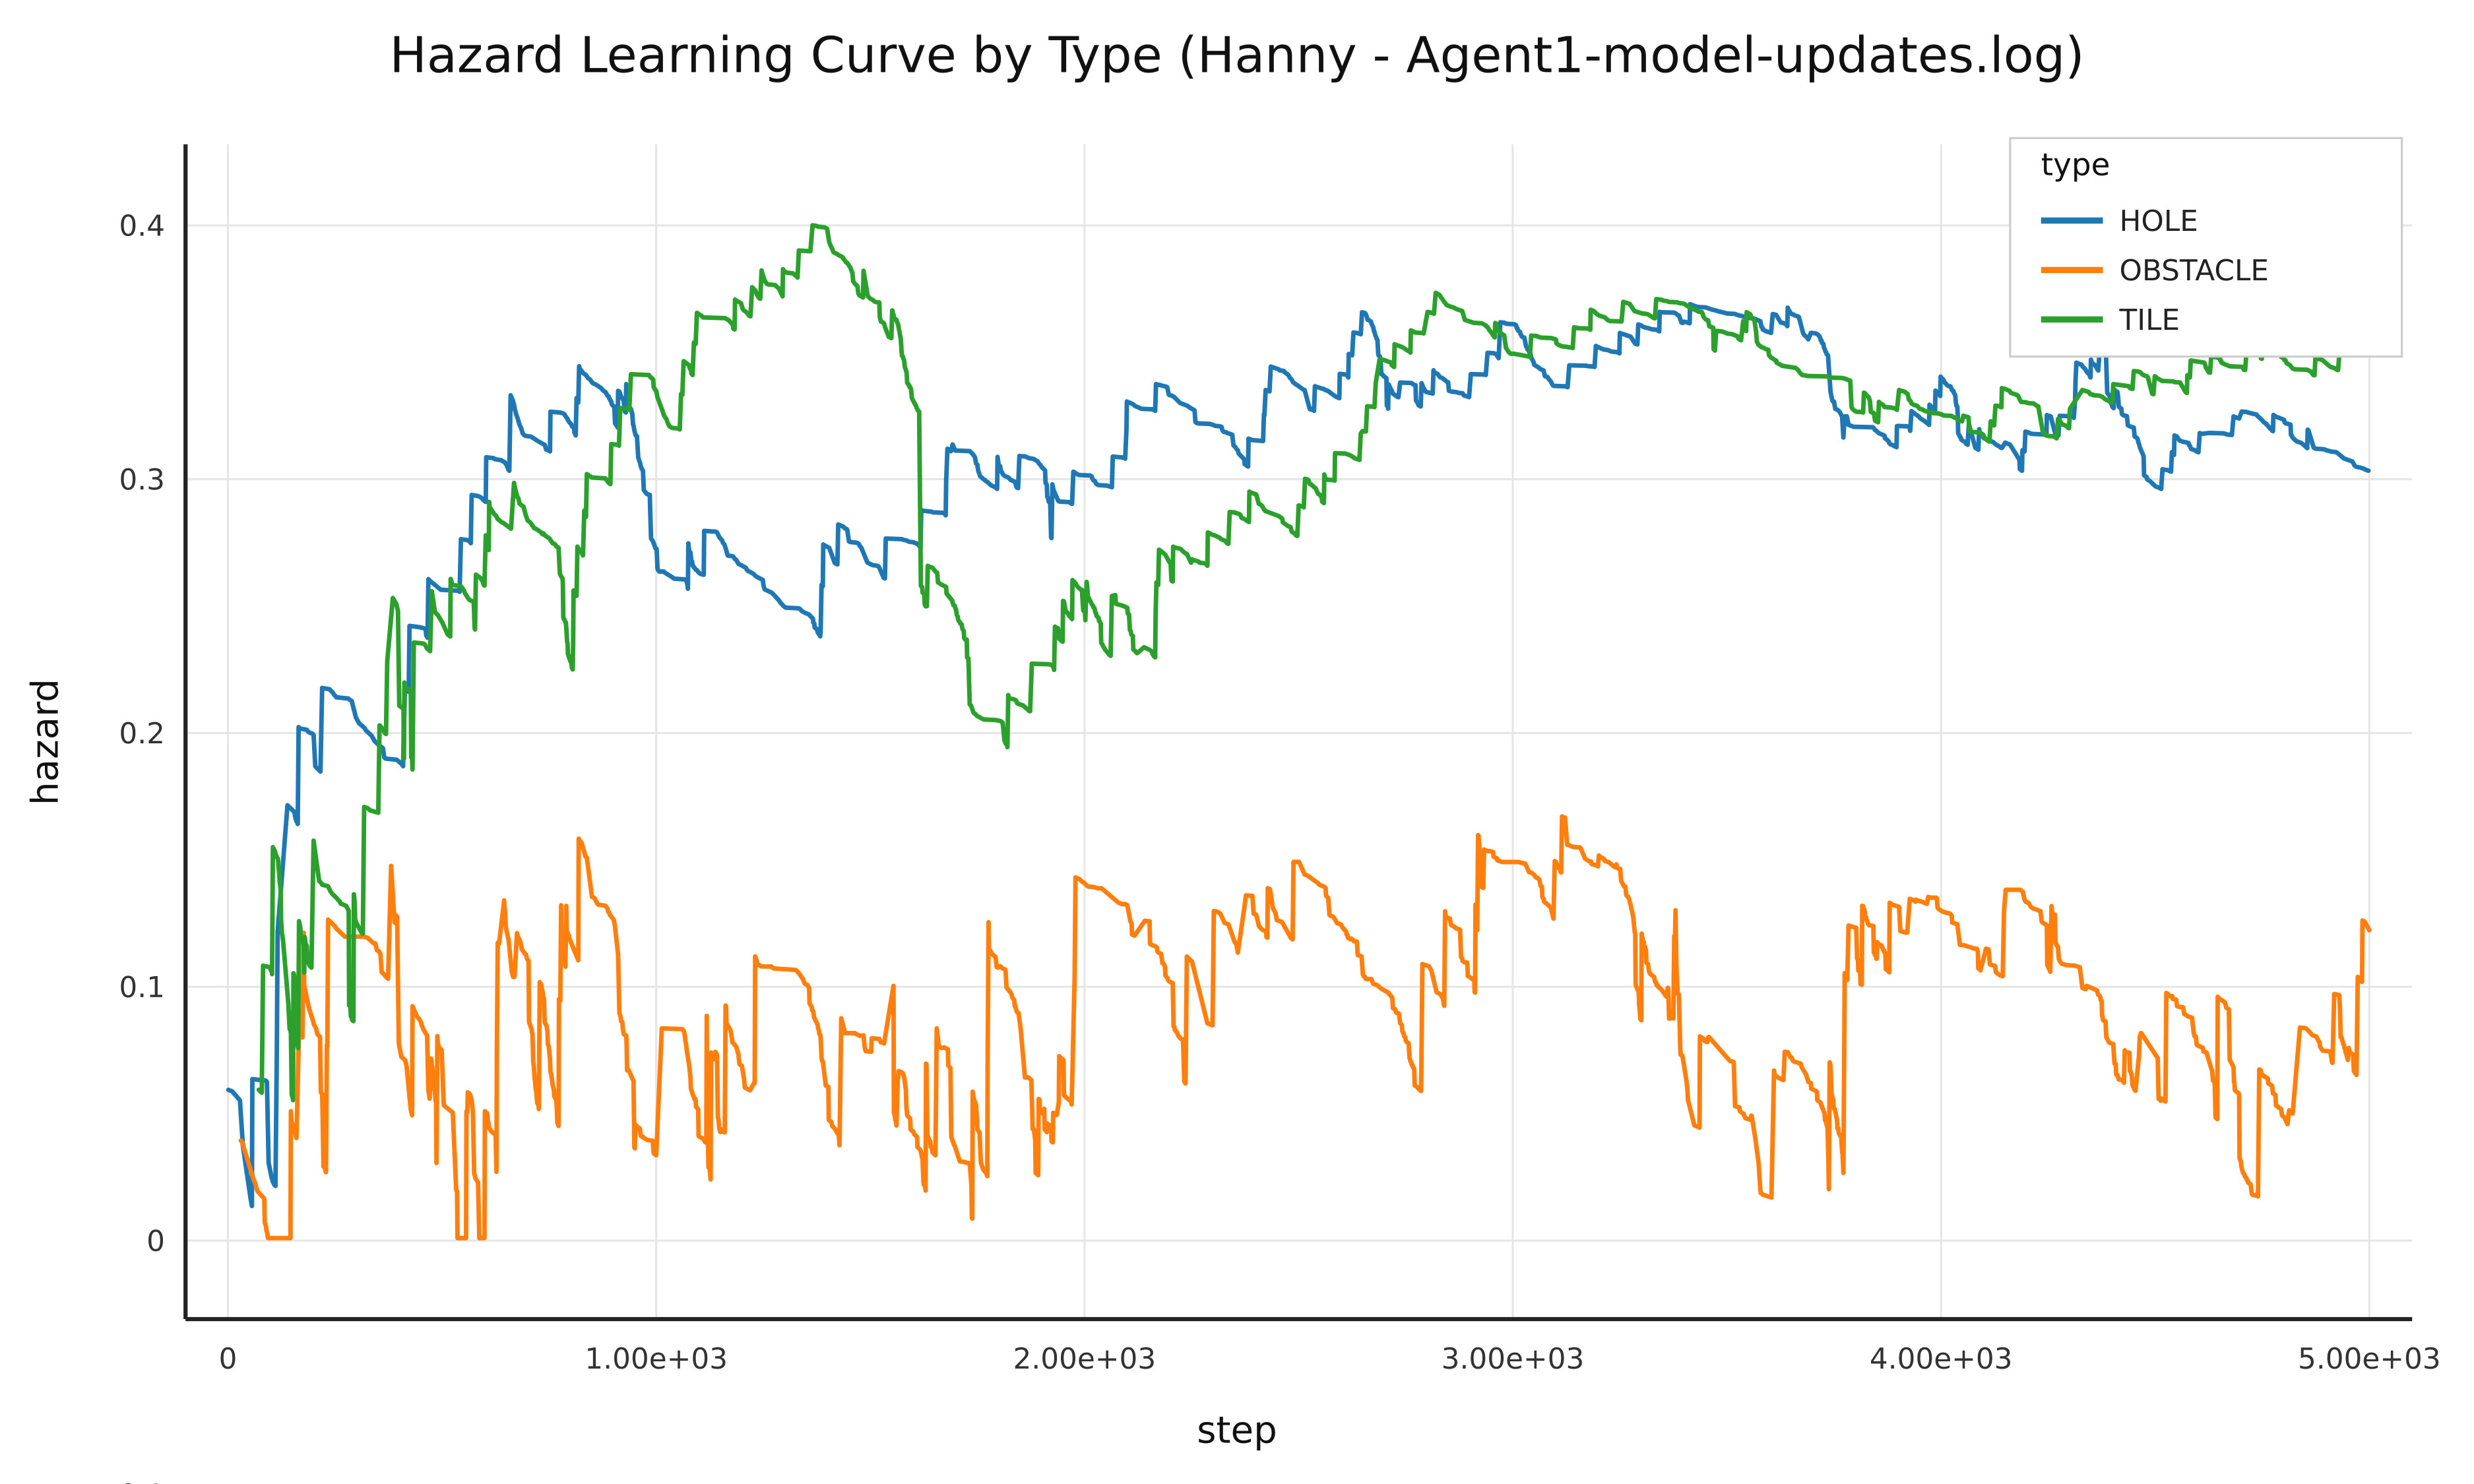
\includegraphics[width=\linewidth]{5000Steps_Para1.jpg}
        \caption{\(\lambda\) vs Steps - Parameters 1}
        \label{hzd-para1}
    \end{subfigure}
    \hfill
    \begin{subfigure}[b]{0.31\linewidth}
        \centering
        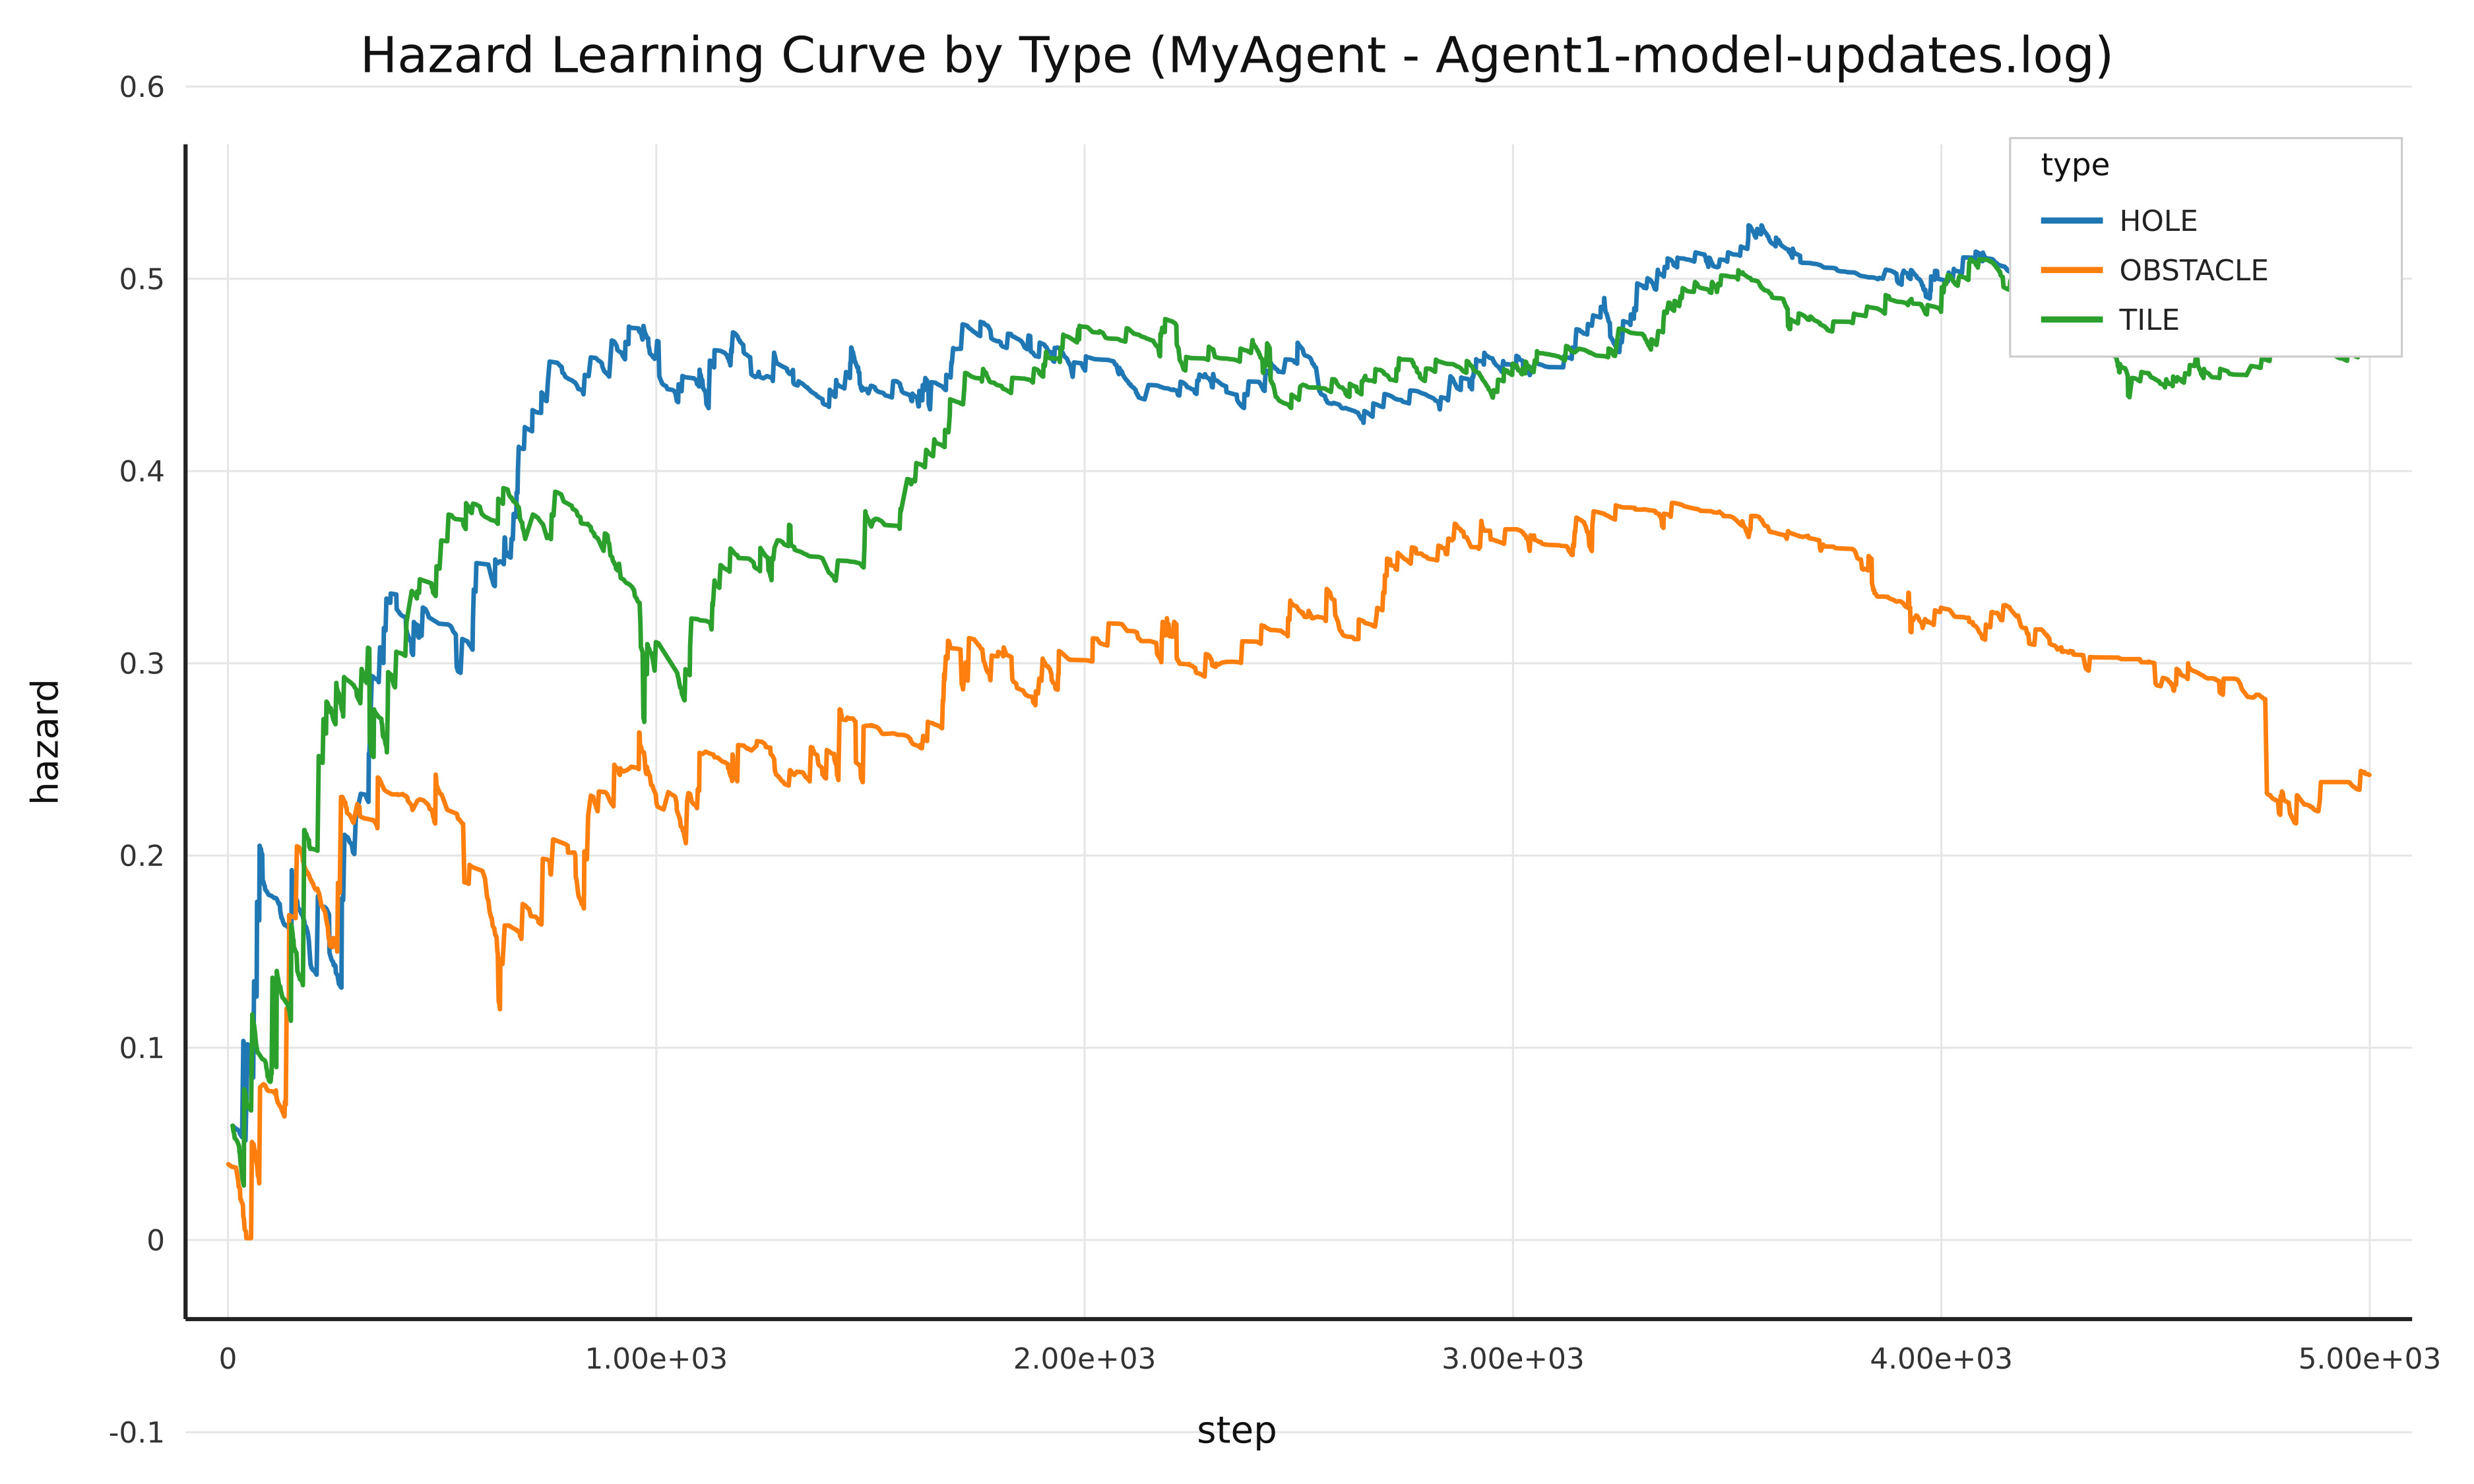
\includegraphics[width=\linewidth]{5000Steps_Para2.jpg}
        \caption{\(\lambda\) vs Steps - Parameters 2}
        \label{hzd-para2}
    \end{subfigure}
    \hfill
    \begin{subfigure}[b]{0.31\linewidth}
        \centering
        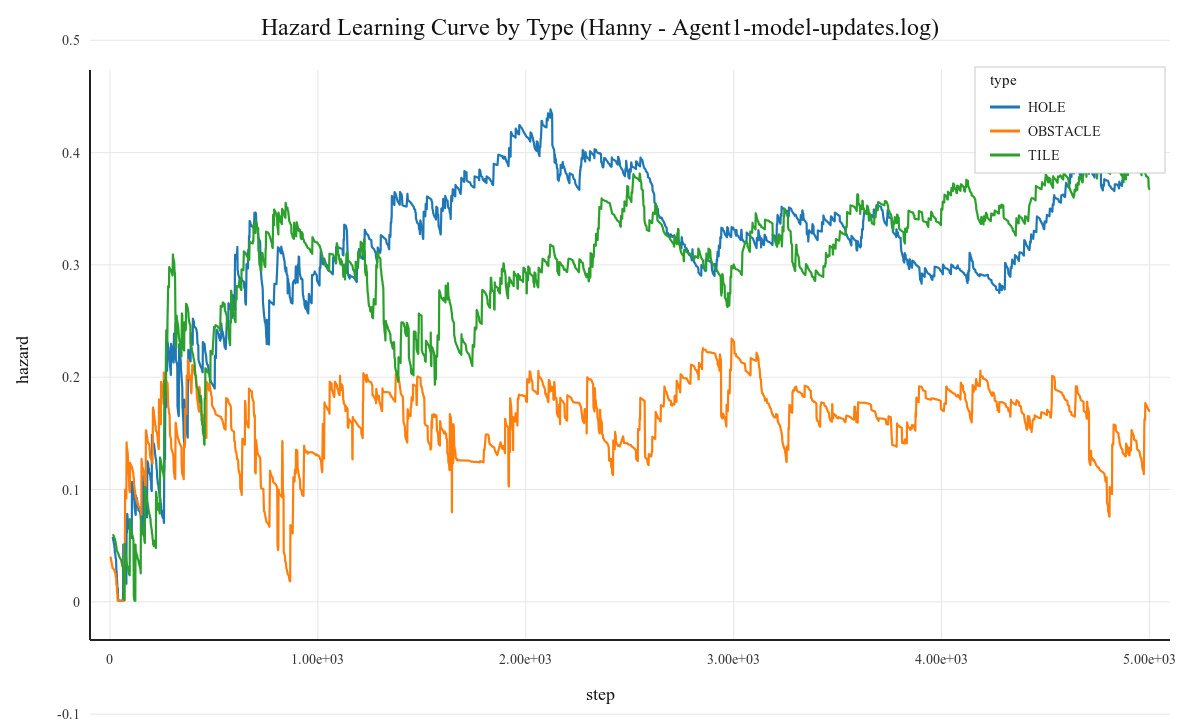
\includegraphics[width=\linewidth]{5000Steps_Para3.jpg}
        \caption{\(\lambda\) vs Steps - Parameters 3}
        \label{hzd-para3}
    \end{subfigure}
    \caption{Hazard Figure Across Different Environment Settings.}
    \label{hzd-5000steps}
\end{figure}

AgentHanny will then recall objects from memory and form plans with picking up {1...available-carry-space} tiles and filling them to {1...expected-carried-tiles} holes, 
then calculate the expected utility of each plan follows:

\[
EU_{plan}
= \sum_{pickup}{p_{tile-alive} \cdot 0.20}
+ \sum_{fill}{p_{hole-alive} \cdot 1.00}
- 0.07 \cdot Distance
- FuelPenalty
\]

The planner enumerates feasible target sequences (with carry-capacity constraints and depth limit), then chooses the plan with the highest expected utility.
If failed to recall any possible plan options, do exploration to make actions continious and systematic.

\paragraph{Communications}
Agent Hanny follows the protocol defined in \texttt{Group7AgentBase} and consumes team messages each think cycle. It uses:
Target lock is acquired/kept for the \emph{current execution target} (not for every recalled target at plan creation time), renewed before expiry, and released when target is completed, invalidated, pre-empted, or when mode switches (e.g., refuel/re-plan).

\paragraph{Memory Layer}
In order to make the online MLE in planning phase possible, AgentHanny keeps a memory side-card to record additional information that original \texttt{TWAgentWorkingMemory} does not provide.
Additional information includes object type, first seen time, last seen time, and whether the object spawning is observed, providing a hybrid object-survival estimation mode (probabilistic for unobserved-spawn objects and deterministic lifetime branch for observed-spawn objects).
This side card is always synchronized with the original working memory, and the information is updated when new observation is made or the object is observed by the team.

\paragraph{Exploration}
In order to maximize the social welfare, AgentHanny is designed to explore the sections of the tileworld map that are least explored by the team.
To be more specific, AgentHanny divides the map into a dynamic \(n \times n\) grid, where
\[
n = \max\left(1,\left\lfloor \frac{\min(\text{width},\text{height})}{15}\right\rfloor\right).
\]
Each section is scored with negative signals from teammate density, explored coverage, and distance from current position. 
Sections whose center has a too-long distance from AgentHanny is excluded. The section with the best score is selected, and if no valid section exists, the agent falls back to zig-zag exploration.

\subsection{Agent 2 - <Role / Name>}
% Describe objective, local policy, planner, memory, strengths/weaknesses.

\lipsum[1] % placeholder

\subsection{Agent 3 - <Role / Name>}
% Describe objective, local policy, planner, memory, strengths/weaknesses.

\lipsum[1] % placeholder

\subsection{Agent 4 - <Role / Name>}
% Describe objective, local policy, planner, memory, strengths/weaknesses.

\lipsum[1] % placeholder

\subsection{Agent 5 - <Role / Name>}
% Describe objective, local policy, planner, memory, strengths/weaknesses.

\lipsum[1] % placeholder

\subsection{Agent 6 - <Role / Name>}
% Describe objective, local policy, planner, memory, strengths/weaknesses.

\lipsum[1] % placeholder

\section{Agent Communication \& Collaboration}

% Describe:
% - what information is broadcast
% - recipient conventions if any
% - task allocation strategy
% - conflict avoidance
% - how agents share discovered tiles / holes / obstacles / fuel stations
% - whether communication is synchronous or opportunistic
% - how collaboration changes over time

\lipsum[1] % placeholder

\section{Result and Analysis}

% Include:
% - quantitative results across configurations
% - comparison between agent variants or team strategies
% - visualizations/tables if needed
% - interpretation: what worked, what failed, why
% - discussion of trade-offs such as specialization vs flexibility

\lipsum[1] % placeholder

\section{Conclusion}

% Summarize:
% - what your team built
% - key findings
% - major limitations
% - possible future improvements

\lipsum[1] % placeholder

%Bibliography
\bibliographystyle{unsrt}  
\bibliography{references}  


\end{document}
